%%%%%%%%%%%%%%%%%%%%%%%%%%%%%%%%%%%%%%%%%
% Short Sectioned Assignment
% LaTeX Template
% Version 1.0 (5/5/12)
%
% This template has been downloaded from:
% http://www.LaTeXTemplates.com
%
% Original author:
% Frits Wenneker (http://www.howtotex.com)
%
% License:
% CC BY-NC-SA 3.0 (http://creativecommons.org/licenses/by-nc-sa/3.0/)
%
%%%%%%%%%%%%%%%%%%%%%%%%%%%%%%%%%%%%%%%%%

%----------------------------------------------------------------------------------------
%	PACKAGES AND OTHER DOCUMENT CONFIGURATIONS
%----------------------------------------------------------------------------------------

\documentclass[paper=a4, fontsize=11pt]{scrartcl} % A4 paper and 11pt font size

\usepackage[T1]{fontenc} % Use 8-bit encoding that has 256 glyphs
%\usepackage{fourier} % Use the Adobe Utopia font for the document - comment this line to return to the LaTeX default
\usepackage[english]{babel} % English language/hyphenation
\usepackage{amsmath,amsfonts,amsthm} % Math packages
\usepackage{bm}
\usepackage{lipsum} % Used for inserting dummy 'Lorem ipsum' text into the template
\usepackage{graphicx} % This one is for pictures
\usepackage{sectsty} % Allows customizing section commands
\allsectionsfont{\centering \normalfont\scshape} % Make all sections centered, the default font and small caps
\usepackage{color}
\usepackage{float}
\floatplacement{figure}{H}
\usepackage{fancyhdr} % Custom headers and footers
\pagestyle{fancyplain} % Makes all pages in the document conform to the custom headers and footers
\fancyhead{} % No page header - if you want one, create it in the same way as the footers below
\fancyfoot[L]{} % Empty left footer
\fancyfoot[C]{} % Empty center footer
\fancyfoot[R]{\thepage} % Page numbering for right footer
\renewcommand{\headrulewidth}{0pt} % Remove header underlines
\renewcommand{\footrulewidth}{0pt} % Remove footer underlines
\setlength{\headheight}{13.6pt} % Customize the height of the header

%\numberwithin{equation}{section} % Number equations within sections (i.e. 1.1, 1.2, 2.1, 2.2 instead of 1, 2, 3, 4)
%\numberwithin{figure}{section} % Number figures within sections (i.e. 1.1, 1.2, 2.1, 2.2 instead of 1, 2, 3, 4)
%\numberwithin{table}{section} % Number tables within sections (i.e. 1.1, 1.2, 2.1, 2.2 instead of 1, 2, 3, 4)

%\setlength\parindent{0pt} % Removes all indentation from paragraphs - comment this line for an assignment with lots of text

%----------------------------------------------------------------------------------------
%	TITLE SECTION
%----------------------------------------------------------------------------------------

\newcommand{\horrule}[1]{\rule{\linewidth}{#1}} % Create horizontal rule command with 1 argument of height

\title{	
\normalfont \normalsize 
\textsc{Columbia University -- Fall 2013} \\ [25pt] % Your university, school and/or department name(s)
\horrule{0.5pt} \\[0.4cm] % Thin top horizontal rule
\huge Machine Learning Homework \#5\\ % The assignment title
\horrule{2pt} \\[0.5cm] % Thick bottom horizontal rule
}

\author{Joe Ellis - jge2105} % Your name

\date{\normalsize\today} % Today's date or a custom date

\begin{document}

\maketitle % Print the title

%----------------------------------------------------------------------------------------
%	PROBLEM 1
%----------------------------------------------------------------------------------------

\section{Problem 1}
Assume you are a contestant of a game show in which you are presented with three closed doors A, B, and C. 
Behind one of the doors is a car which will be yours if you choose the right door. 
After you have randomly (as you have no prior information) selected a door (say door A), the game host opens door B which has nothing inside, while keeping door A and C closed. 
The host then asks whether you want to change your selection from A to C. 
Should you change?

We should change, and the following rational should describe why.
Let's assume WLOG that we choose a door, and model our choice based on the random variable $X$.  
The door with the actual prize behind it will be modeled by the random variable $W$, and the door chosen by the host of the show will be model another random variable $Y$.
Let's try to make a graphical model based on these random variables.  
First, we know that $X$ is not directly dependent on $W$, because I have no possible way to know the state of $W$.
Therefore, in a directed graphical model, we know that there is no connection between these two nodes.
However, $Y$ (the door that the host chooses) is directly effected by the value of $X$ (the door I choose), and $W$, the actual winning door. 
Therefore, we have a unidirected model with connections from $X$ to $Y$ and $W$ to $Y$.

So our first choice of a door or $X$ is made with no knowledge of $Y$, therefore based on slide 12 of lecture 15, because $Y$ is unseen. 
We have $X \perp W$.
Which means that our choice of $X$ is completely independent of the actual winning door, and therefore each door has an equal shot of holding the winning prize.  
Since there are 3 doors, and we choose each equally and each has an equal shot of containing the prize the likely hood of our choice $X$ resulting in the prize is $\frac{1}{3}$.

However, after we have seen the value of $Y$, $X$ and $W$ are no longer independent.
In fact, 

%----------------------------------------------------------------------------------------
%	PROBLEM 2
%----------------------------------------------------------------------------------------

\section{Problem 2}
\subsection{Problem 2a}
We want to prove that $X \perp Y|Z$ if and only if the joint probability $p(x,y,z)$ can be expressed in the form of $a(x,z)b(y,z)$.
\paragraph{PROOF}
Assume that $X \perp Y|Z$, therefore we know that $p(x|y,z) = p(x,z)$ and $p(x|y) \neq p(x)$.

\begin{align}
p(x,y,z) &= p(y,z)p(x|y,z) \\
&= p(y,z)p(x,z).
\end{align}

Therefore, we have $p(x,y,z)$ can be expressed in the form of $a(x,z)b(y,z)$.

\subsection{Problem 2b}
 We want to prove or disprove with a counter example, that $X \perp Y|Z$ and $X \perp W|(Y,Z)$ implies that $X \perp (W,Y)|Z$.
We want to use this knowledge to prove that $p(x|(w,y,z)) = p(x|z)$.

\paragraph{PROOF}
\begin{align}
p(x|(w,y,z)) &= p(x|y,z),\ by \ X \perp W|(Y,Z) \\
&= p(x|z), \ by \  X \perp Y|Z.
\end{align}

Thus, we have shown $X \perp (W,Y)|Z$.

\subsection{Problem 2c}

\subsection{Bonus}

%----------------------------------------------------------------------------------------
%	PROBLEM 3
%----------------------------------------------------------------------------------------

\section{Problem 3}
Using the given graphical model we would like to find Walle.  
Let's create a junction tree based on the given graphical model of Walle.
Each step in creation of the graphical model will be represented by a figure describing the work done. 

The first step is moralization, which is completed by attaching nodes that both have the same child.  This can be seen in figure ~\ref{fig:moralization}.

\begin{figure}
\centering
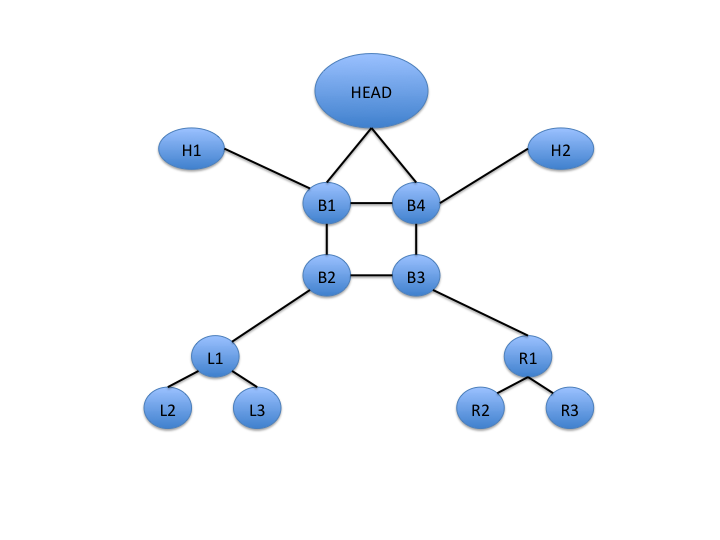
\includegraphics[width=0.5\textwidth]{Problem3/Slide1.png}
\caption{Moralization of the directed graph into an undirected graph}
\label{fig:moralization}
\end{figure}

We then triangulate the graph by placing a connection between node B2 and B4, as shown in figure ~\ref{fig:trig}

\begin{figure}
\centering
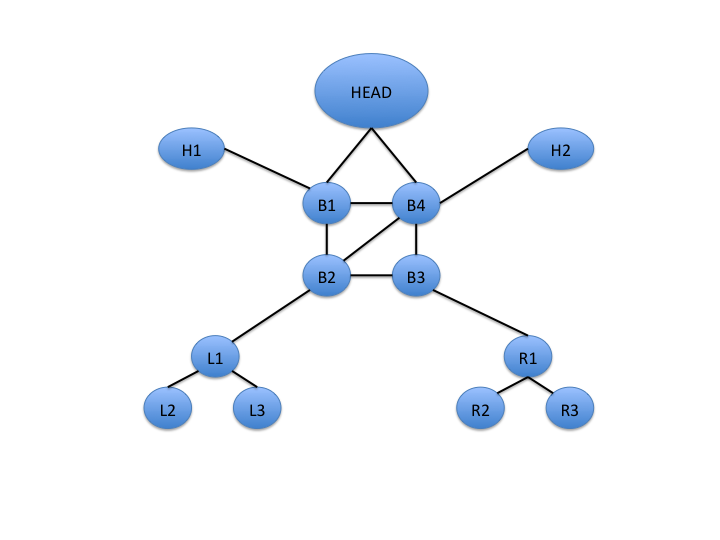
\includegraphics[width=0.5\textwidth]{Problem3/Slide2.png}
\caption{Triangulated graph of Wall-E}
\label{fig:trig}
\end{figure}

After this we then find the maximal cliques over the triangulated graphs, and the cliques can be seen in figure ~\ref{fig:clique}.

\begin{figure}
\centering
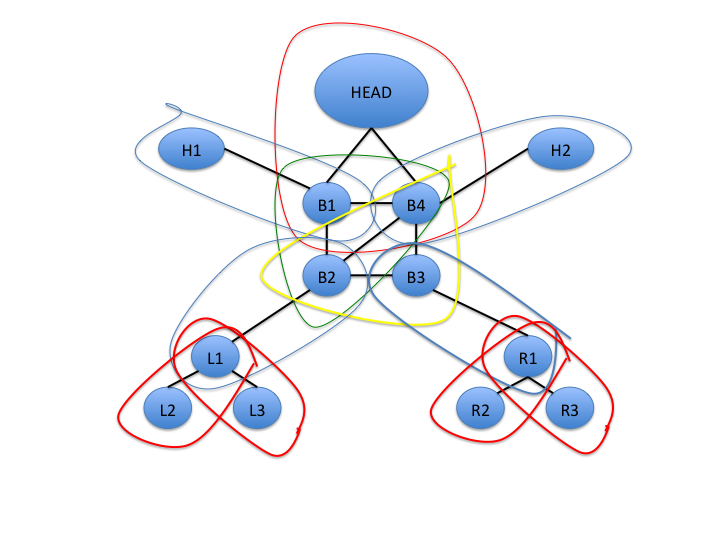
\includegraphics[width=0.5\textwidth]{Problem3/Slide3.png}
\caption{Maximal Cliques over the graph of Wall-E}
\label{fig:clique}
\end{figure}

Once we have the maximal cliques use Kruskal's algorithm in two stages to connect up the Junction Tree.  
We begin by connecting the nodes with seperators with the highest cardinality, which happen to be 2.
These seperators and there connections can be seen in figure ~\ref{fig:ver1}.

\begin{figure}
\centering
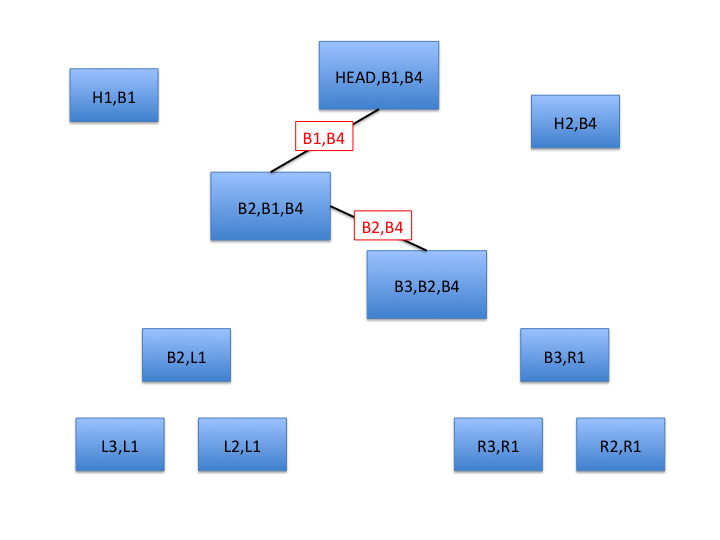
\includegraphics[width=0.5\textwidth]{Problem3/Slide4.png}
\caption{Nodes connected in Kruskal's algorithm with most seperator cardinality}
\label{fig:ver1}
\end{figure}

Then we connect the nodes using Kruskal's algorithm with seperator cardinality of 1, as long as the connection does not create a cycle, working down from the connections that are already present. 
The results of this can be seen in figure ~\ref{fig:ver2}, and the root node is the node containing elements B3,B2,B4.

\begin{figure}
\centering
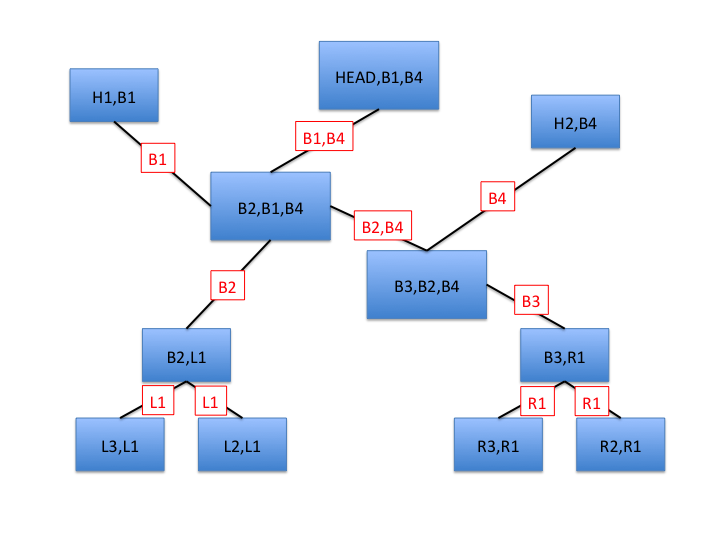
\includegraphics[width=0.5\textwidth]{Problem3/Slide5.png}
\caption{Final junction tree created using Kruskal's algorithm}
\label{fig:ver2}
\end{figure}
%----------------------------------------------------------------------------------------
%	PROBLEM 4
%----------------------------------------------------------------------------------------

\section{Problem 4}
In this problem we will analyze how the Junction Tree Algorithm is applied to a markov chain.
I have created a matlab script that allows the 





\end{document}